\documentclass[a4paper,12pt]{article}

\usepackage{escexam}

%\excludecomment{solution}

%\renewcommand*\ttdefault{cmvtt}
\setlength{\headheight}{85.05003pt}
\begin{document}

%\vspace*{14ex}

\makeheader{1}                              					% examination number (used to set theorem, lemma numbers)
           {September 11, 2026}      					         		% examination date or deadline
					 {60}											% total marks
					 {Homework Assignment 1}							% Minor Quiz 1, Major Quiz 2, End sem, etc
					
%\begin{tabular}{cl}
%1. & This question paper contains a total of 12 pages (13 sides of paper). Please verify.\\
%2. & Write your name, roll number, department, section on \textbf{every side of every sheet} of this booklet\\
%3. & Write final answers \textbf{neatly} in the given boxes.\\
%%4. & Do not give derivations/elaborate steps unless the question specifically asks you to provide these.
%\end{tabular}


\begin{problem}{}
(10 points)

\smallskip 
\noindent
(a) Construct a Simulink model of the helicopter control system shown in the figure below. 
\begin{center}
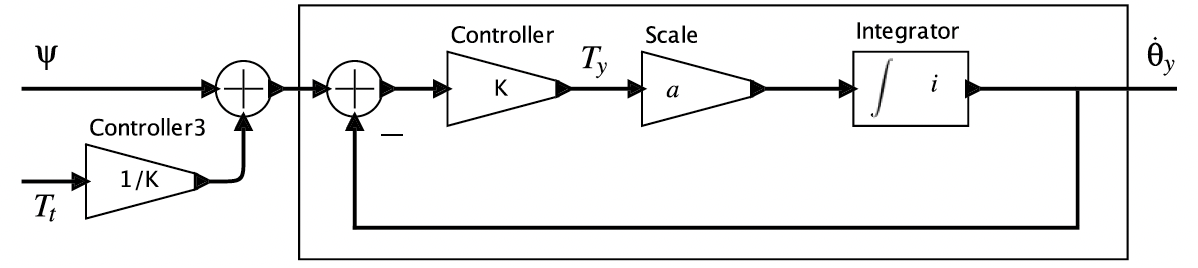
\includegraphics[scale=0.65]{helicopter.png}
\end{center}
Choose some reasonable parameters and plot the actual angular velocity as a function of time, assuming that the desired angular velocity is zero, $\psi(t) = 0$, and that the top-rotor torque is non-zero, $T_t(t) = bu(t)$.
Give your plot for three different values of $K$ and discuss how the behavior varies with $K$.

\smallskip
\noindent
(b) Modify the model of part (a) to replace the Controller (the simple scale-by-K actor) with the alternative controller shown in the figure below. 
\begin{center}
\includegraphics[scale=0.65]{PI_Controller.png}
\end{center}
This alternative controller is called a proportional-integrator (PI) controller. It has two parameters $K_1$ and $K_2$. 
Experiment with the values of these parameters, give some plots of the behavior with the same inputs as in part~(a), and
discuss the behavior of this controller in contrast to the one of part~(a).\\
\ \\
\begin{minipage}{1\textwidth}
       \rectangle{\linewidth}{24cm}
		%\ruledrectangle{7}
        
\end{minipage}
\newpage
\ \\
\begin{minipage}{1\textwidth}
        \rectangle{\linewidth}{24cm}
		%\ruledrectangle{7}
\end{minipage}
\newpage
\ \\
\begin{minipage}{1\textwidth}
		\rectangle{\linewidth}{24cm}
		%\ruledrectangle{7}
\end{minipage}
\newpage
\ \\
\begin{minipage}{1\textwidth}
        \rectangle{\linewidth}{24cm}
		%\ruledrectangle{7}
\end{minipage}
\end{problem}



\newpage

\begin{problem}{}
(10 points) 

\smallskip
\noindent
The states of the linearized model of a vehicle steering system represent the lateral deviation of the vehicle from the x-axis and the angle between the vehicle axis and the $x$-axis. The output of the linearized model is only the first state. Construct a Simulink model for the vehicle steering system with its controller that includes an observer. The dynamics are available in Example 6.4 and Example 7.3 in [AM09]. Apply a sinusoidal signal as the reference trajectory that specifies the desired deviation of the vehicle from the x-axis with time. Plot the output (lateral deviation of the vehicle from the x-axis) with time. 

\smallskip
\noindent
[AM09] K. J. Astrom and R. M. Murray. Feedback Systems: An Introduction for Scientists and Engineers. Princeton University Press, 2009. \\
http://www.cds.caltech.edu/~murray/books/AM08/pdf/am08-complete\_22Feb09.pdf . \\
\\
\begin{minipage}{1\textwidth}
        \rectangle{\linewidth}{19cm}
		  %\ruledrectangle{7
\end{minipage}
\newpage
\ \\
\begin{minipage}{1\textwidth}
        \rectangle{\linewidth}{24cm}
		%\ruledrectangle{7}
\end{minipage}
\newpage
\ \\
\begin{minipage}{1\textwidth}
		\rectangle{\linewidth}{24cm}
		%\ruledrectangle{7}
\end{minipage}
\newpage
\ \\
\begin{minipage}{1\textwidth}
        \rectangle{\linewidth}{24cm}
		%\ruledrectangle{7}
\end{minipage}
\end{problem}


\newpage

\begin{problem}{}
(10 points) 

\smallskip
\noindent
Consider the following model for a thermostat system.

\begin{center}
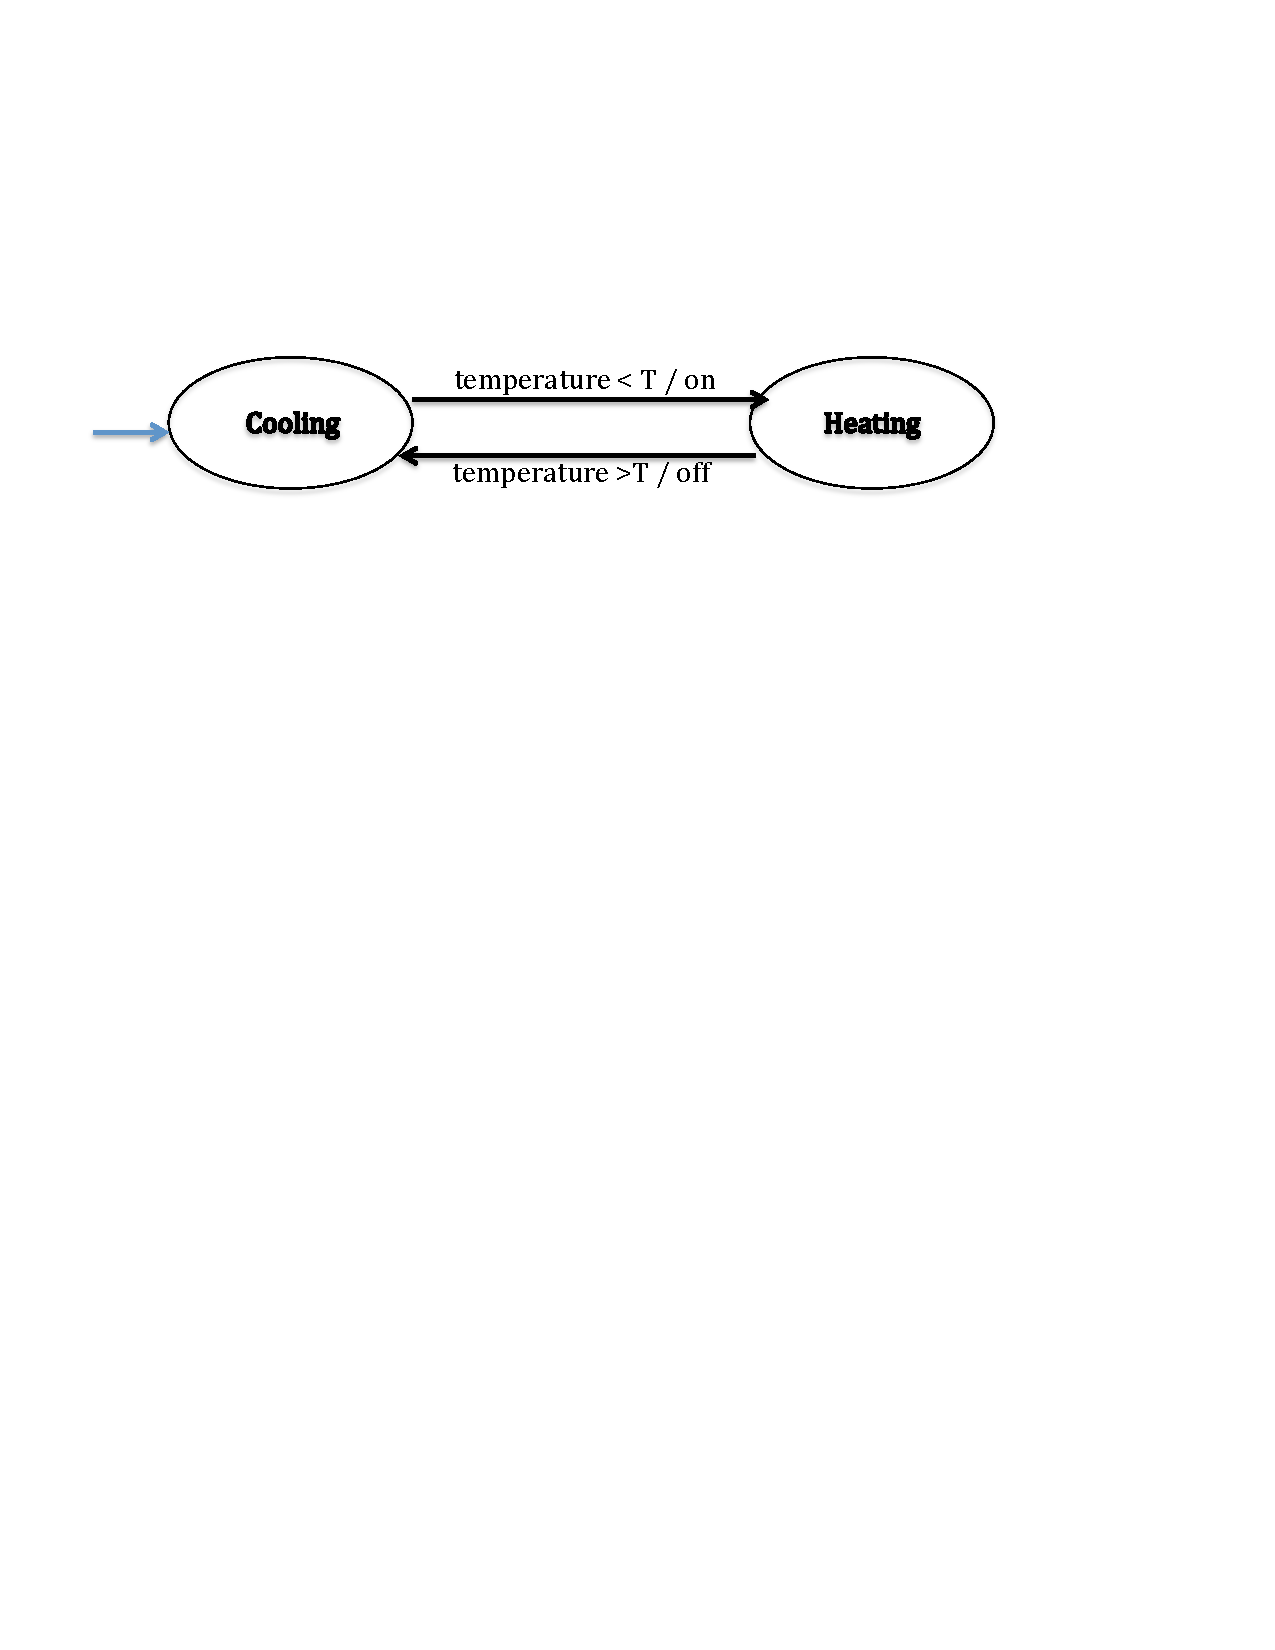
\includegraphics[scale=0.5]{temperature.pdf}
\end{center}

The thermostat has been designed to maintain the temperature of a room at T$^{\circ}$C.
The model has two states: \textit{cooling} and \textit{heating}.
When the system is in the \textit{cooling} state and the temperature of the room goes below T$^{\circ}$C, the system
generates a signal to switch on a heater and moves to the \textit{heating} state. 
When the temperature of the room goes over T$^{\circ}$C, the system generates a signal to switch off the heater and moves to
the \textit{cooling} state.\\
(a) Represent the system as an actor that takes the current temperature as input and produces a signal to control the heater. The actor uses the set point T as a parameter.\\
(b) Identify a design problem in the model.\\
(c) Provide two different remedies to address the problem. \\
(d) Compare your proposed two solutions in terms of ease of implementation and guarantees on the system behavior.  \\
\\
\begin{minipage}{1\textwidth}
        \rectangle{\linewidth}{16cm}
		  %\ruledrectangle{7}
\end{minipage}
\newpage
\ \\
\begin{minipage}{1\textwidth}
        \rectangle{\linewidth}{24cm}
		%\ruledrectangle{7}
\end{minipage}
\newpage
\ \\
\begin{minipage}{1\textwidth}
		\rectangle{\linewidth}{24cm}
		%\ruledrectangle{7}
\end{minipage}
\newpage
\ \\
\begin{minipage}{1\textwidth}
        \rectangle{\linewidth}{24cm}
		%\ruledrectangle{7}
\end{minipage}
\end{problem}


\newpage

\begin{problem}{}
(10 points) 

\smallskip
\noindent
Construct a timed automation model of a thermostat where the heater will be switched on when the room temperature is less than 22C and switched off when the temperature is above 26C. We also have the following additional requirement. Before switching on or off, it will generate a ``beep'' sound every second for 5 seconds as a warning. That means once the system senses that the temperature is less than 22C, it will generate the warning first, and then the heater will be switched on. Similarly, a warning sound will be issued before switching off the heater after the temperature reaches 26C.
\\
\\
\begin{minipage}{1\textwidth}
        \rectangle{\linewidth}{20cm}
		  %\ruledrectangle{7}
\end{minipage}
\newpage
\ \\
\begin{minipage}{1\textwidth}
        \rectangle{\linewidth}{24cm}
		%\ruledrectangle{7}
\end{minipage}
\newpage
\ \\
\begin{minipage}{1\textwidth}
		\rectangle{\linewidth}{24cm}
		%\ruledrectangle{7}
\end{minipage}
\newpage
\ \\
\begin{minipage}{1\textwidth}
        \rectangle{\linewidth}{24cm}
		%\ruledrectangle{7}
\end{minipage}
\end{problem}

\newpage

\begin{problem}{}
(10 points) 

\smallskip
\noindent
Consider the following synchronous composition of two state machines A and B.

\begin{center}
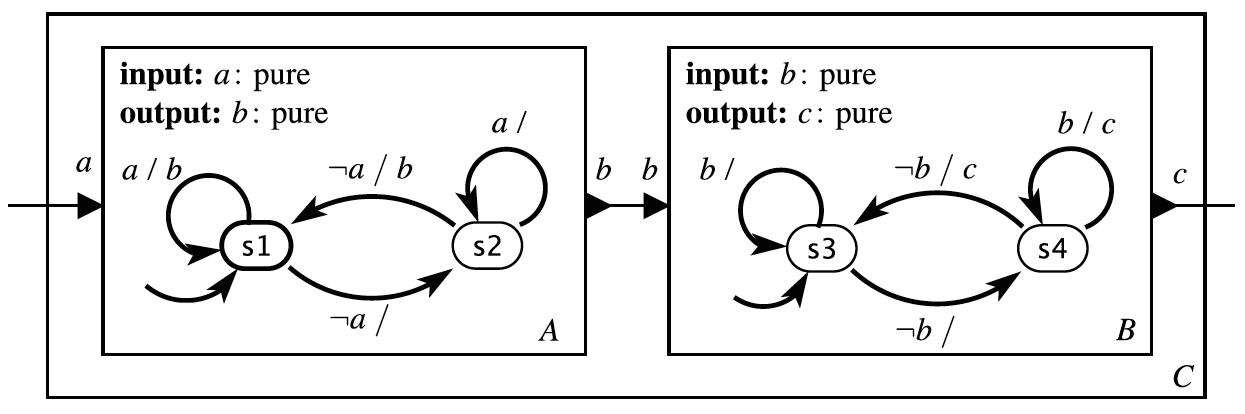
\includegraphics[scale=0.5]{composition.png}
\end{center}

Construct a single state machine C representing the composition. 
Which states of the composition are unreachable?
\\
\\
\\
\begin{minipage}{1\textwidth}
        \rectangle{\linewidth}{20cm}
		  %\ruledrectangle{7}
\end{minipage}
\newpage
\ \\
\begin{minipage}{1\textwidth}
        \rectangle{\linewidth}{24cm}
		%\ruledrectangle{7}
\end{minipage}
\newpage
\ \\
\begin{minipage}{1\textwidth}
		\rectangle{\linewidth}{24cm}
		%\ruledrectangle{7}
\end{minipage}
\newpage
\ \\
\begin{minipage}{1\textwidth}
        \rectangle{\linewidth}{24cm}
		%\ruledrectangle{7}
\end{minipage}
\end{problem}


\newpage

\begin{problem}{}
(10 points) 

\smallskip
\noindent
Consider the following SDF model:

\begin{center}
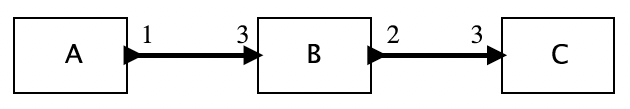
\includegraphics[scale=0.5]{sdf.png}
\end{center}
The numbers adjacent to the ports indicate the number of tokens produced or consumed by
the actor when it fires. Answer the following questions about this model.

(a) Let $q_A$, $q_B$, and $q_C$ denote the number of firings of actors $A$, $B$, and $C$, respectively. Write
down the balance equations and find the least positive integer solution. 

(b) Find a schedule for an unbounded execution that minimizes the buffer sizes on the two
communication channels. What is the resulting size of the buffers?
\\
\\
\begin{minipage}{1\textwidth}
        \rectangle{\linewidth}{18cm}
		  %\ruledrectangle{7}
\end{minipage}
\newpage
\ \\
\begin{minipage}{1\textwidth}
        \rectangle{\linewidth}{24cm}
		%\ruledrectangle{7}
\end{minipage}
\newpage
\ \\
\begin{minipage}{1\textwidth}
		\rectangle{\linewidth}{24cm}
		%\ruledrectangle{7}
\end{minipage}
\newpage
\ \\
\begin{minipage}{1\textwidth}
        \rectangle{\linewidth}{24cm}
		%\ruledrectangle{7}
\end{minipage}
\end{problem}


\end{document}